\pagenumbering{arabic}
\setcounter{page}{1}
\subsection*{Context}

Because of their capacity of innovation, hackers and other malware writers will always be one step ahead of antiviruses or any other kind of protection tool. According to PurpleSec \cite{purplesec}, the number of malware infections have significantly increased over the last ten years and reached a total of 812.76 millions in 2018. With approximately 230 000 new malware every day, companies spend on average \$ 2.4 million on defenses against such malicious software.

Malware detection is one of the most serious challenges in system security nowadays. Two techniques exist to perform malware analysis: \textit{static} and \textit{dynamic} analyses. The first one involves examining the sample without actually running or executing the code. This is mainly achieved by disassembling or determining the signature of the binary file. Dynamic analysis operates by running the code in a controlled environment, like a sandbox, and observing its behaviour. While dynamic analysis proposes a more thorough kind of analysis, the cost of starting and running a sandbox is significant. On the other hand, static analysis can easily be evaded by using a method known as \textit{packing}.

\subsection*{What is packing ?}

Packing is a widely used strategy that enables executable files to bypass static analysis. It includes various methods that compress or encrypt the content of a given file. It also appends a \textit{stub} section containing the routine that will be executed at runtime for decompression. While it can be used by benign executables in order to avoid reverse-engineering, WildList states that 92\% of packed executables hide harmful programs.

Figure \ref{fig:packing_process} illustrates the life-cycle of a program being packed and loaded into memory. The original file is encrypted or compressed and then stored in the packed sections of the new executable. Another section is also added, containing the decompression routine. When the file is run, this decompression \textit{stub} will decompress the packed sections before the file is actually loaded into memory. The file eventually carries on its execution as if it were never packed.

\begin{figure}[!ht]
\centering
  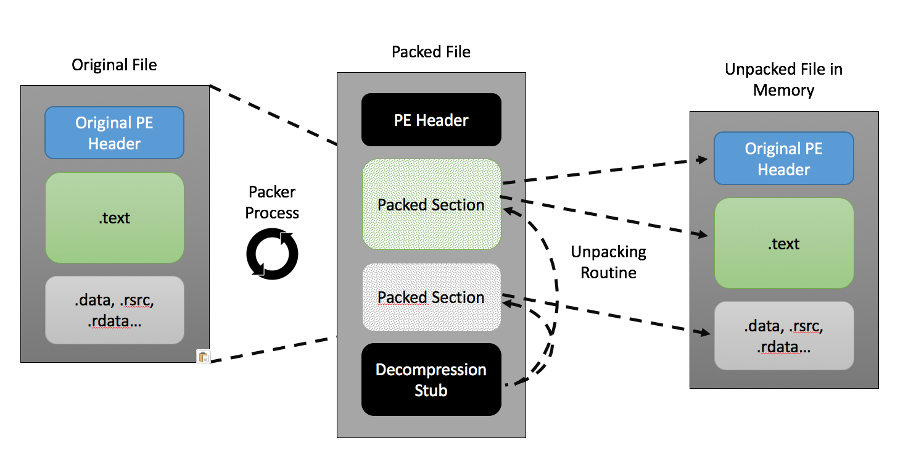
\includegraphics[width=\linewidth]{Figures/packing_process.png}
  \caption{Life-cycle of a packed binary \cite{mc_afee}}
  \label{fig:packing_process}
\end{figure}

\subsection*{Challenges}

Detecting whether a potential malware is packed constitutes a crucial step towards actual packer detection and malware identification. If this initial process fails, then further static analysis will also fail and dynamic analysis will need to take over the detection process, resulting in substantial time overheads. The first challenge is therefore to achieve packing detection within a reasonable period of time.

As new varieties of malware emerge every day, new packing techniques are also frequently developed. Let it be by the use of private or self-created tools, packed malware also bypass signature-based detection by applying multi-layer packing. It simply consists of packing the same file numerous times using the same or different packers, which is sufficient to alter the content of the file and disturb static detectors. Being able to stay on track with the evolution of this ecosystem is also a serious second challenge.

Another issue relies in the collection of packed samples. Static detectors mainly rely on signatures to identify packed executables, such binary files being extracted from a huge previously created database. Each of them is labeled to learn rules and distinguish if, and in the best situation, how a potential malware has been packed. These databases, used for ground truths generation, are not always accessible and even when they are, their accuracy is hard to assess. A major third challenge is therefore to collect, label and learn correctly over a large panel of samples in order to generalise and capture as many singularities as possible. This will lead to better detection rules, and thus sharper decision abilities.

\subsection*{Solution}

Our approach is similar to the method developed by Perdisci et al. \cite{perdisci_classification_2008} in their paper : efficiently distinguish if an executable is packed such that only those files are sent to a universal unpacker. Combined with a fast and efficient static malware detector such as the one proposed by Baldangombo et al. \cite{baldangombo_static_2013}, a complete malware detection system going from packing identification to malware classification could emerge, offering high-end performance in record time. Regarding the structure, we will follow the same logic as Biondi et al. \cite{biondi_effective_2019}. We will use various machine-learning algorithms over custom and assumed accurate ground truths in order to build an online tool that detects whether a given PE file is packed. PE refers to \textit{Portable Executable} which is the format for executables used in 32-bit and 64-bit versions of Windows operating systems. Using the same approach, we will also consider feature selection to enhance computation times and proceed to economical analysis as an assessment of stability over time.

To achieve this, we first combine multiple existing packing detectors to help us create a super decision maker able to correctly label any PE file. Combined with the feature extraction tool used by Biondi et al. \cite{biondi_effective_2019}, we continuously supply a database with features from executables that are kindly provided by Cisco. The database is therefore filled with \texttt{(features, label)} pairs that correspond to PE files. By the means of a modular ground truth generator, we create various kinds of datasets that are fed to a total of 10 different machine learning algorithms. Each combination of classifiers, parameters and features is tested to keep only the scenarios providing the best prediction power. An economical analysis is also performed to assess their stability over time. At the end, the best classifier is retained. Through a web interface, any user can then select a file and our detection system will identify if it is packed with an average accuracy of 99.5\% in less than 50 ms.

\subsection*{Structure}

The remainder of this document is structured as follows. In section \ref{related_works}, previously proposed implementations in the context of packing detection and classification are studied. Section \ref{methods} gathers how we found and combined existing detection tools to create our own detector. The database and ground truths generation are also described in this section. Section \ref{preprocessing} shows how the different data were processed or converted to meet our needs. Thenceforth, the complete machine learning process is explained in section \ref{machine_learning}, covering the identification of the detection problem up to the election of the final best classifier. After that, the online tool is briefly exposed in section \ref{online_tool}. Eventually, all the work is summarised and a final conclusion with further improvements is exposed in section \ref{conclusion}.